% \chapter{Background}

% Our starting point is, for any positive integer $d \in \field{N}$, the
% Cartesian products:
% \begin{equation*}
% \field{R}^d = \field{R} \times \overset{(d)}{\dotsm} \times \field{R} =\{ (x_1, \dotsc, x_d) : x_k \in \field{R} \text{ for } 1\leq k \leq d\}.
% \end{equation*}
% These sets, endowed with the operations of addition and scalar multiplication, have the structure of a \emph{vector field}:
% \begin{description}
% 	\item[Addition] For $\x = (x_1, \dotsc, x_d), \y = (y_1, \dotsc, y_d) \in \field{R}^d$, 
% 	\begin{equation*}
% 	\x + \y = (x_1+y_1, \dotsc, x_d+y_d) \in \field{R}^d.
% 	\end{equation*}
% 	\item[Scalar multiplication] For $\x \in \field{R}^d$ and $\lambda \in \field{R}$, 
% 	\begin{equation*}
% 	\lambda \cdot \x = \lambda \x = (\lambda x_1, \dotsc, \lambda x_d) \in \field{R}^d.
% 	\end{equation*}
% \end{description}
% Given $\x, \y, \z \in \field{R}^d$, $\lambda, \mu \in \field{R}$,
% \begin{enumerate}
% 	\item The addition is commutative: $\x + \y = \y + \x$.
% 	\item Existence of identity elements for addition: Let $\boldsymbol{0} = (0, \dotsc, 0)$. $\x + \boldsymbol{0} = \x$. 
% 	\item The addition is associative: $\x + (\y + \z) = (\x + \y) + \z$.
% 	\item Existence of inverse elements for addition: If $\x = (x_1, \dotsc, x_d)$, the element $-\x = (-x_1, \dotsc, -x_d)$ satisfies $\x + (-\x) = \boldsymbol{0}$.  We write $\x - \y$ instead of $\x + (-\y)$.
% 	\item Scalar multiplication is compatible with field multiplication: $\lambda (\mu \x) = (\lambda \mu) \x$.
% 	\item Existence of identity for scalar multiplication: $1 \cdot \x = \x$.
% 	\item Scalar multiplication is distributive with respect to addition: $\lambda (\x + \y) = \lambda \x + \lambda \y$.
% 	\item Scalar multiplication is distributive with respect to field addition: $(\lambda + \mu)\x = \lambda \x + \mu\x$.
% \end{enumerate}
% A \emph{basis} of $\field{R}^d$ is any finite set $\{ \boldsymbol{b}_k : 1\leq k \leq d \}$ satisfying two properties:
% \begin{description}
% \item [Spanning property] For all $\x \in \field{R}^d$ there exist $d$ scalars $\{ \lambda_1, \dotsc, \lambda_d \}$ so that $\x = \sum_{k=1}^d \lambda_k \boldsymbol{b}_k$.
% \item [Linear independence] If $\{ \lambda_1, \dotsc, \lambda_d\}$ satisfy $\sum_{k=1}^d \lambda_k \boldsymbol{b}_k = \boldsymbol{0}$, then it must be $\lambda_k=0$ for all $1\leq k \leq d$.
% \end{description}

% \begin{problem}\label{problem:basisRd}
% Define in $\field{R}^d$, for each $1\leq k \leq d$, the element $\e_k$ to be the ordered $d$-tuple with $k$-th entry equal to one, and zeros on all other entries.
% \begin{enumerate}
% 	\item Prove that $\{ \e_k : 1\leq k \leq d\}$ is a basis for $\field{R}^d$.
% 	\item Set $\boldsymbol{b}_k = \e_k - \e_{k+1}$ for $1\leq k < d$, $\boldsymbol{b}_d = \e_d$.  Is $\{ \boldsymbol{b}_k : 1\leq k \leq d\}$ a basis for $\field{R}^d$?
% \end{enumerate}
% \end{problem}

% \section{Functions}

% Given sets $X, Y$, we define a \emph{function} $f\colon X \to Y$ to be a subset of $X \times Y$ subject to the following condition: for every $\x \in X$ there is exactly one element $\y \in Y$ such that the ordered pair $(\x, \y)$ is contained in the subset defining $f$. The sets $X$ and $Y$ are called respectively the \emph{domain} and \emph{codomain} of $f$.  

% If $A$ is any subset of the domain $X$, then $f(A)$ is the subset of the codomain $Y$ consisting of all images of elements of $A$. We say that $f(A)$ is the \emph{image} of $A$ under $f$. The set $f(X)$ is called the image of $f$.

% If $Y \subseteq \field{R}$, we say that the function $f$ is real-valued.  For a real-valued function $f\colon \field{R}^d \to \field{R}$, we may regard the corresponding ordered pairs $(\x, y) \in \field{R}^d\times\field{R}$ as points in a $(d+1)$--dimensional space.  We call this set the \emph{graph} of $f$.

% The \emph{inverse image} of a subset $B$ of the codomain $Y$ under a function $f$ is the subset of the domain $X$ defined by $f^{-1}(B) = \{ \x \in X : f(x) \in B\}$.

% For sets $X, Y, Z$, the \emph{function composition} of $f\colon X \to Y$ with $g\colon Y \to Z$ is the function $g\circ f\colon X \to Z$ defined by $\big( g \circ f \big)(\x) = g \big( f(\x) \big)$.

% \begin{example}[Linear Functions]\label{example:linearFunction}
% We say that a function $f \colon \field{R}^{d_1} \to \field{R}^{d_2}$ is \emph{linear} if it preserves the operations in $\field{R}^{d_1}$: 
% \begin{equation*}
% f(\x + \lambda \y) = f(\x) + \lambda f(\y) \text{ for }\x, \y \in \field{R}^d, \lambda \in \field{R}.
% \end{equation*}

% With this definition, the functions $f\colon \field{R} \to \field{R}$ given by $f(x) = 3x$ is indeed a linear function, but $g\colon \field{R} \to \field{R}$ given by $g(x)=3x+5$ is not!  
% It is not hard to see that the only real-valued linear constant function $f\colon \field{R} \to \field{R}$ is $f(x) = 0$ (since $f(0)=f(x-x)=f(x)-f(x)=0$).  For a non-constant real-valued linear function $f\colon \field{R} \to \field{R}$, it is also easy to see that the image is the whole real line.  Indeed:

% There exists $x_0\neq 0$ so that $f(x_0)=y_0\neq 0$. For any $y \in \field{R}$, choose $x = y x_0/y_0$.  We have then
% \begin{equation*}
% f(x) = f\big( \tfrac{y}{y_0} x_0 \big) = \tfrac{y}{y_0} f(x_0) = y.
% \end{equation*}
% \end{example}

% \begin{example}[Convex Functions]\label{example:convexFunction}
% A subset $C \subseteq \field{R}^d$ is said to be \emph{convex} if for every $\x, \y \in C$, and every $\lambda \in [0,1]$, the point $\lambda \x + (1-\lambda) \y$ is also in $C$.   Given such a convex set, we say that a real-valued function $f \colon C \to \field{R}$ is \emph{convex} if 
% \begin{equation*}
% f\big(\lambda \x + (1-\lambda)\y\big) \leq \lambda f(\x) + (1-\lambda) f(\y)
% \end{equation*}
% \begin{figure}[ht!]
% 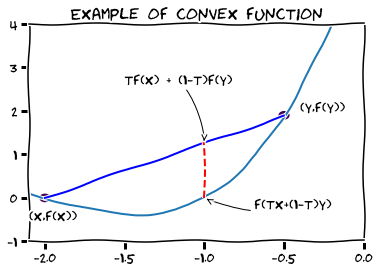
\includegraphics[width=0.5\linewidth]{convexFunction.png}
% \caption{In convex functions, the segment joining two points of the graph is always above the graph.}
% \label{figure:convexFunction}
% \end{figure}
% If instead we have $f\big(\lambda \x + (1-\lambda)f(\y)\big) < \lambda f(\x) + (1-\lambda) f(\y)$ for $0<\lambda<1$, we say that the function is \emph{strictly convex}.  A function $f$ is said to be \emph{concave} (resp.~\emph{strictly concave}) if $-f$ is convex (resp.~strictly convex).
% \end{example}

\begin{example}[Posynomials]\label{example:posynomial}
Consider the set $\mathfrak{P}_d = \{ (x_1, \dotsc, x_d) \in \field{R}^d : x_k > 0 \text{ for } 1\leq k \leq d\}$. A function $f \colon \mathfrak{P}_d \to \field{R}$ is said to be a \emph{posynomial} if it can be written in the form of a linear combination with non-negative coefficients of products of powers of non-negative variables.  More formally: $f$ is a posynomial if there exists $n \in \field{N}$, $n$ positive constants $\{ c_j : 1 \leq j \leq n \}$ and $n \times d$ arbitrary real exponents $\{ \alpha_{jk} : 1\leq j \leq n, 1 \leq k \leq d \}$ so that 
\begin{equation*}
f(\x) = \sum_{j=1}^n c_j \prod_{k=1}^d x_k^{\alpha_{jk}}.
\end{equation*}
Notice that the domain of a given posynomial may not be extended in general anywhere else in $\field{R}^d$.  For example, notice the obvious restrictions for the function $f\colon \mathfrak{P}_2 \to \field{R}$ given by $f(x_1,x_2) = x_1\sqrt{x_2} + \frac{\pi}{x_1}$.
\end{example}

% \begin{example}[Rosenbrock Functions]\label{example:Rosenbrock2}
% Given strictly positive parameters $a,b > 0$, consider the $(a,b)$--Rosenbrock function $\mathcal{R}_{a,b}\colon \field{R}^2 \to \field{R}$ defined by:
% \begin{equation*} 
% \mathcal{R}_{a,b}(x_1, x_2) = (a-x_1)^2 + b(x_2-x_1^2)^2.
% \end{equation*}
% It is easy to see that Rosenbrock functions are multi-variate polynomials (prove it!).  The image of $\mathcal{R}_{a,b}$ is the interval $[0,\infty)$.  Indeed, note first that $\mathcal{R}_{a,b}(\x) \geq 0$ for all $\x \in \field{R}^2$.  Zero is attained: $\mathcal{R}_{a,b} (a,a^2) = 0$.  Note also that $\mathcal{R}_{a,b}(0,x_2) = a^2 + bx_2^2$ is a polynomial of degree 2, hence unbounded for $x_2 \in \field{R}$.

% Figure \ref{figure:Rosenbrock} illustrates a contour plot with several level lines of $\mathcal{R}_{1,1}$ on the domain $D = [-2,2] \times [-1,3]$, as well as its graph
% \begin{figure}[ht!]
% \begin{tabular}{cc}
% 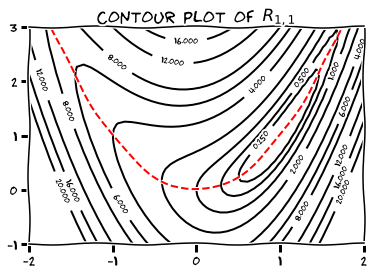
\includegraphics[width=0.5\linewidth]{rosenbrockContour} &
% 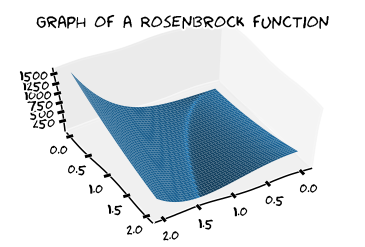
\includegraphics[width=0.5\linewidth]{rosenbrockGraph}
% \end{tabular}
% \caption{Details of the graph of $\mathcal{R}_{1,1}$}
% \label{figure:Rosenbrock}
% \end{figure}
% \end{example}

% This is a good spot to introduce the goal of these notes.  The main purpose of \emph{optimization} is the search for \emph{extrema} of real-valued functions.  Given a set $D \subseteq \mathbb{R}^d$, and a real-valued function $f\colon D \to \field{R}$, we say that a point $\xstar \in D$ is:
% \begin{enumerate}
% 	\item A \emph{global minimum} for $f$ on $D$ if $f(\xstar) \leq f(\x)$ for all $\x \in D$.
% 	\item A \emph{global maximum} for $f$ on $D$ if $f(\xstar) \geq f(\x)$ for all $\x \in D$.
% 	\item A \emph{strict global minimum} for $f$ on $D$ if $f(\xstar) < f(\x)$ for all $\x \in D \setminus \{ \xstar \}$.
% 	\item A \emph{strict global maximum} for $f$ on $D$ if $f(\xstar) > f(\x)$ for all $\x \in D \setminus \{ \xstar \}$.
% 	\item A \emph{local minimum} for $f$ on $D$ if there exists $\delta>0$ so that  $f(\xstar) \leq f(\x)$ for all $\x \in B_\delta(\xstar)\cap D$.
% 	\item A \emph{local maximum} for $f$ on $D$ if there exists $\delta>0$ so that  $f(\xstar) \geq f(\x)$ for all $\x \in B_\delta(\xstar)\cap D$.
% 	\item A \emph{local minimum} for $f$ on $D$ if there exists $\delta>0$ so that  $f(\xstar) < f(\x)$ for all $\x \in B_\delta(\xstar)\cap D$, $\x \neq \xstar$.
% 	\item A \emph{local maximum} for $f$ on $D$ if there exists $\delta>0$ so that  $f(\xstar) > f(\x)$ for all $\x \in B_\delta(\xstar)\cap D$, $\x \neq \xstar$.
% \end{enumerate}

% Let's play around with some more examples of functions, before we proceed to techniques for finding extrema:

% \begin{problem}[Linear Functions]\label{problem:LinearFunctions-d2d}
% Let $\boldsymbol{A} = \big[ a_{jk} \big]_{j,k=1}^d$ be a square matrix with real coefficients.  Considering elements in $\field{R}^d$ as horizontal matrices, and by means of matrix multiplication, we construct functions $\mathcal{L}_{\boldsymbol{A}} \colon \field{R}^d \to \field{R}^d$ and $\mathcal{R}_{\boldsymbol{A}} \colon \field{R}^d \to \field{R}^d$ given by
% \begin{align*}
% \mathcal{L}_{\boldsymbol{A}}(\x) &= \begin{bmatrix} x_1 \dotsb x_d \end{bmatrix} \begin{bmatrix} a_{11} &\dotsb &a_{1d} \\ \vdots & \ddots & \vdots \\ a_{d1} &\dotsb &a_{dd} \end{bmatrix} \\
% \mathcal{R}_{\boldsymbol{A}}(\x) &= \begin{bmatrix} a_{11} &\dotsb &a_{1d} \\ \vdots & \ddots & \vdots \\ a_{d1} &\dotsb &a_{dd} \end{bmatrix} \begin{bmatrix} y_1 \\ \vdots \\ y_d \end{bmatrix}
% \end{align*}
% Prove that these two are linear functions.
% \end{problem}

% \begin{problem}
% Prove that, if $\boldsymbol{A}$ is a symmetric matrix, then $\mathcal{L}_{\boldsymbol{A}}(\x) = \mathcal{R}_{\boldsymbol{A}}(\x)$ for all $\x \in \field{R}^d$.
% \end{problem}

% \begin{example}[Bilinear Forms]\label{example:BilinearForm}
% Under the same conditions as in problem \ref{problem:LinearFunctions-d2d}, we construct functions $\bilinear{A} \colon \field{R}^d \times \field{R}^d \to \field{R}$ given by
% \begin{equation*}
% \bilinear{A}(\x, \y) = \begin{bmatrix} x_1 \dotsb x_d \end{bmatrix} \begin{bmatrix} a_{11} &\dotsb &a_{1d} \\ \vdots & \ddots & \vdots \\ a_{d1} &\dotsb &a_{dd} \end{bmatrix} \begin{bmatrix} y_1 \\ \vdots \\ y_d \end{bmatrix}
% \end{equation*}
% We call functions constructed in this way \emph{bilinear forms}.
% \end{example}

% \begin{problem}\label{problem:BilinearForm}
% Prove that, if the associated matrix is symmetric ($\boldsymbol{A} = \transpose{\boldsymbol{A}}$), then $\bilinear{A}(\x,\y) = \bilinear{A}(\y,\x)$ for all $\x, \y \in \field{R}^d$.
% \end{problem}

% \begin{example}[Quadratic Forms]\label{example:QuadraticForm}
% Each symmetric bilinear form has an associated \emph{quadratic form}: A function $\quadratic{A} \colon \field{R}^d \to \field{R}$ constructed as follows:
% \begin{equation*}
% \quadratic{A}(\x) = \bilinear{A}(\x,\x) = \begin{bmatrix} x_1 \dotsb x_d \end{bmatrix} \begin{bmatrix} a_{11} &\dotsb &a_{1d} \\ \vdots & \ddots & \vdots \\ a_{1d} &\dotsb &a_{dd} \end{bmatrix} \begin{bmatrix} x_1 \\ \vdots \\ x_d \end{bmatrix}
% \end{equation*}
% We say that the quadratic form (or the associated matrix) is:
% \begin{description}
% \item[positive definite] if $\quadratic{A}(\x) > 0$ for all $\x \in \field{R}^d \setminus \{ \boldsymbol{0} \}$.
% \item[positive semidefinite] if $\quadratic{A}(\x)\geq 0$ for all $\x \in \field{R}^d$.
% \item[negative definite] if $\quadratic{A}(\x) < 0$ for all $\x \in \field{R}^d \setminus \{ \boldsymbol{0} \}$.
% \item[negative semidefinite] if $\quadratic{A}(\x) \leq 0$ for all $\x \in \field{R}^d$.
% \item[indefinite] if there exist $\x, \y \in \field{R}^d$ so that $\quadratic{A}(\x) \quadratic{A}(\y) < 0$. 
% \end{description}
% \end{example}

% \begin{problem}
% Give examples of $2 \times 2$ symmetric matrices that are positive definite, positive semidefinite, negative definite, negative semidefinite, and indefinite.
% \end{problem}

% \begin{problem}
% Prove that a symmetric $2\times 2$ matrix $\boldsymbol{A} = \big[ \begin{smallmatrix} a_{11} & a_{12} \\ a_{21} & a_{22} \end{smallmatrix} \big]$ is positive definite if and only if $a_{11}>0$ and $\det(\boldsymbol{A})>0$.
% \end{problem}

% \begin{problem}[Principal Minors]\label{problem:PrincipalMinors}
% Given a general square matrix $\boldsymbol{A}$, we define for each $1\leq \ell \leq d$, $\Delta_\ell$ (the $\ell$th \emph{principal minor} of $\boldsymbol{A}$) to be the determinant of the upper left-hand corner $\ell \times \ell$--submatrix of $\boldsymbol{A}$.  
% \begin{center}
% \begin{tikzpicture}
% \draw (0,0) node{%
% $\begin{bmatrix}
% a_{11} & a_{12} & a_{13} & \dotsb & a_{1n} \\
% a_{21} & a_{22} & a_{23} & \dotsb & a_{2n} \\
% a_{31} & a_{32} & a_{33} & \dotsb & a_{3n} \\
% \vdots & \vdots & \vdots & \ddots & \vdots \\
% a_{n1} & a_{n2} & a_{n3} & \dotsb & a_{nn} 
% \end{bmatrix}$};
% \draw[dashed] (-2, 0.73) -- (-1.35, 0.73) -- (-1.35, 1.2) node[above]{$\Delta_1$};
% \draw[dashed] (-2, 0.27) -- (-0.5, 0.27) -- (-0.5, 1.2) node[above]{$\Delta_2$};
% \draw[dashed] (-2, -0.15) -- (0.4, -0.15) -- (0.4, 1.2) node[above]{$\Delta_3$};
% \end{tikzpicture}
% \end{center}
% Prove that a symmetric matrix $\boldsymbol{A}$ is positive definite if and only if $\Delta_\ell > 0$ for all $1\leq \ell \leq d$.
% %\item Negative definite if and only if $(-1)^\ell \Delta_\ell>0$ for all $1\leq \ell \leq d$.
% \end{problem}

% \begin{example}[Inner products]\label{example:innerprod}
% We say that a symmetric bilinear form $\bilinear{A}$ is an \emph{inner product} if its associated quadratic form is positive definite.  By extension, we call an inner product any function $\mathcal{F} \colon \field{R}^d \times \field{R}^d \to \field{R}$ that satisfies the following four properties for all $\x, \y, \z \in \field{R}^d, \lambda \in \field{R}$:
% \begin{enumerate}
% \item $\mathcal{F}(\x+\y, \z) = \mathcal{F}(\x, \z) + \mathcal{F}(\y, \z)$.
% \item $\mathcal{F}(\lambda \x, \y) = \lambda \mathcal{F}(\x, \y)$.
% \item $\mathcal{F}(\x, \y) = \mathcal{F}(\y, \x)$.
% \item $\mathcal{F}(\x, \x) \geq 0$, $\mathcal{F}(\x, \x) = 0$ if and only if $\x = \boldsymbol{0}$.
% \end{enumerate}
% \end{example}

% \begin{problem}\label{problem:innerprodRd}
% Prove that $\langle \cdot, \cdot \rangle \colon \field{R}^d \times \field{R}^d \to \field{R}$ given by
% \begin{equation*}
% \langle \x, \y \rangle = \sum_{k=1}^d x_k y_k
% \end{equation*}
% is an inner product.
% \end{problem}

% \begin{problem}\label{problem:real-valuedLinearFunction}
% Prove that, if $f\colon \field{R}^d \to \field{R}$ is a real-valued linear function, then there exist a unique $\boldsymbol{a}_0 \in \field{R}^d$ so that $f(\x)=\langle \boldsymbol{a}_0, \x \rangle$ for all $\x \in \field{R}^d$.
% \end{problem}

% \begin{problem}\label{problem:affineFunction}
% We say that $\tau\colon \field{R}^d \to \field{R}^d$ is a translation if there exist a fixed $\x_0 \in \field{R}^d$ so that $\tau(\x) = \x + \x_0$ for all $\x \in \field{R}^d$.

% An \emph{affine function} $h\colon \field{R}^d \to \field{R}$ is a composition of a real-valued linear function $f\colon \field{R}^d \to \field{R}$ with a translation $\tau\colon \field{R} \to \field{R}$.

% Prove that for each affine function $h$ there exist a unique $\boldsymbol{a}_0 \in \field{R}^d$ and a unique $\lambda_0 \in \field{R}$ so that $h(\x) = \lambda_0 + \langle \boldsymbol{a}_0, \x \rangle$ for all $\x \in \field{R}^d$.  Use this result to prove that the graph of an affine function is a hyperplane in $\field{R}^{d+1}$.
% \end{problem}

% \begin{problem}[Eigenvalues]\label{problem:eigenvalues}
% Given a general square $d \times d$ matrix $\boldsymbol{A}$, consider the function $p_{\boldsymbol{A}} \colon \field{C} \to \field{C}$ given by $p_{\boldsymbol{A}}(\lambda) = \det\big(\boldsymbol{A} - \lambda \boldsymbol{I}_d \big)$.  The solutions (in $\field{C}$) of the equation $p_{\boldsymbol{A}}(\lambda)=0$ are called the \emph{eigenvalues} of $\boldsymbol{A}$.  Prove the following statements:
% \begin{enumerate}
% 	\item $p_{\boldsymbol{A}}$ is a polynomial of (at most) degree $d$ in $\lambda$---we call it the \emph{characteristic polynomial} of $\boldsymbol{A}$.
% 	\item The eigenvalues of a symmetric matrix are all real.
% 	\item If $\lambda \in \field{R}$ is a root  of multiplicity $n$ of the characteristic polynomial of a (non-trivial) symmetric matrix, then there exist $n$ linearly independent vectors $\{ \x_1, \x_2, \dotsc, \x_n \}$ satisfying $\mathcal{L}_{\boldsymbol{A}} (\x_k) = \lambda \x_k$ ($1\leq k \leq n$).
% 	\item If $\lambda_1 \neq \lambda_2$ are different roots of the characteristic polynomial of a symmetric matrix, and $\x_1, \x_2 \in \field{R}^d$ satisfy $\mathcal{L}_{\boldsymbol{A}}(\x_k) = \lambda_k \x_k$ ($k=1,2$), then $\langle \x_1, \x_2 \rangle = 0$.
% 	\item A symmetric matrix is positive definite (resp.~negative definite) if and only if all its eigenvalues are positive (resp.~negative).
% 	\item A symmetric matrix is positive semidefinite (resp.~negative semidefinite) if and only if all its eigenvalues are non-negative (resp.~non-positive)
% 	\item A symmetric matrix is indefinite if there exist two eigenvalues $\lambda_1 \neq \lambda_2$ with different sign.
% \end{enumerate}
% \end{problem}

% \begin{example}[Norms]\label{example:norm}
% A \emph{norm} in $\field{R}^d$ is a function $\norm{\cdot} \colon \field{R}^d \to \field{R}$ that satisfies the following properties:
% For all $\x, \y \in \field{R}^d$, and for all $\lambda \in \field{R}$,
% \begin{enumerate}
% 	\item $\norm{\x} \geq 0$.
% 	\item $\norm{\x} = 0$ if and only if $\x = \boldsymbol{0}$
% 	\item $\norm{ \lambda \x} = \abs{\lambda} \norm{\x}$.
% 	\item Triangle inequality: $\norm{\x + \y} \leq \norm{\x} + \norm{\y}$.
% \end{enumerate}
% \end{example}

% \begin{problem}\label{problem:norm}
% Consider the function $\norm{\cdot} \colon \field{R}^d \to \field{R}$ defined by 
% \begin{equation*}
% \norm{\x} = \langle \x, \x \rangle^{1/2}.
% \end{equation*}
% \begin{enumerate}
% 	\item Prove that $\norm{\cdot}$ is a norm
% 	\item Prove the \emph{Cauchy-Schwartz inequality}: For all $\x, \y \in \field{R}^d$, 
% 	\begin{equation*}
% 	\big\lvert \langle \x, \y \rangle \big\rvert \leq \norm{\x} \norm{\y}.
% 	\end{equation*}
% \end{enumerate}
% \end{problem}


% \section{Topology}
% The norm introduced in Example \ref{example:norm} induces a \emph{metric} $\dist \colon \field{R}^d \times \field{R}^d \to \field{R}^d$ on the space $\field{R}^d$: 
% \begin{equation*}
% \dist(\x,\y) = \norm{\x - \y} \text{ for any }\x, \y \in \field{R}^d.
% \end{equation*}
% Metrics allow us to measure distance between elements.  These are the four main properties of these objects:  Given $\x, \y, \z \in \field{R}^d$,
% \begin{description}
% 	\item[Separation property] $\dist(\x,\y) \geq 0$.
% 	\item[Identity of indiscernibles] $\dist(\x, \y) = 0$ if and only if $\x = \y$.
% 	\item[Symmetry] $\dist(\x, \y) = \dist(\y, \x)$.
% 	\item[Triangle inequality] $\dist(\x,\z) \leq \dist(\x,\y) + \dist(\y,\z)$. 
% \end{description}
% Metric spaces like $\big( \field{R}^d, \dist(\cdot,\cdot) \big)$ inherit a \emph{topology} in a natural manner, as explained below.

% We define the \emph{open ball} of radius $r>0$ about $\x$ as the set $B_d(\x,r) = \big\{ \y \in \field{R}^d : \norm{\x- \y} < r \big\}$.  We say $\x$ is an interior point of $D \subseteq \field{R}^d$ if $\x \in D$ and there exists $r>0$ so that $B_d(\x, r) \subseteq D$.  A subset $G \subseteq \field{R}^d$ is said to be open if all its points are interior.

% A \emph{neighborhood} of the point $\x$ is any subset of $\field{R}^d$ that contains an open ball about $\x$ as subset. 

% A \emph{sequence} $\sequence{\x}{n}$ in $\field{R}^d$ is an enumerated collection of elements of $\field{R}^d$ in which repetitions are allowed.  A sequence is said to \emph{converge} to the limit $\x \in \field{R}^d$ if and only if for every $\varepsilon>0$ there exists $N=N(\varepsilon) \in \field{N}$ so that $\norm{\x_n - \x} < \varepsilon$ for all $n \geq N$.  We write then 
% \begin{equation*}
% \x = \lim_{n\to\infty} \x_n = \lim_n \x_n, \text{ or } \lim_{n\to\infty} \norm{\x_n - \x} = \lim_n \norm{\x_n - \x} = 0.
% \end{equation*}

% We say that $\sequence{\x}{n}$ is a \emph{Cauchy sequence} if for every $\varepsilon>0$ there exists $N = N(\varepsilon) \in \field{N}$ so that for any $m,n \geq N$, $\norm{\x_n - \x_m} < \varepsilon$.  

% \begin{problem}[Completeness of Euclidean spaces]\label{problem:Rdcomplete}
% Prove that all Cauchy sequences converge in $\field{R}^d$ (\textbf{Hint}: this is direct consequence of the completeness of $\field{R}$, which you should also prove).
% \end{problem}

% The complement of an open set is called \emph{closed}. In $\field{R}^d$, all subsets $F$ are closed if and only if they are \emph{sequentially closed}: If $\x_n\in F$ for all $n \in \field{N}$ and $\lim_n \norm{\x_n - \x} = 0$, then $\x \in F$.

% We say $D$ is \emph{bounded} if there exists $M>0$ so that $D \subseteq B_d(\boldsymbol{0}, M)$.  A bounded and closed subset of $\field{R}^d$ is called \emph{compact}.

% \begin{theorem}[Bolzano-Weierstrass]\label{theorem:BolzanoWeierstrass}
% Every sequence in a compact set $K$ contains a convergent subsequence.
% \end{theorem}

% \begin{problem}\label{problem:BolzanoWeierstrass}
% Prove Theorem \ref{theorem:BolzanoWeierstrass} for a closed interval $K=[a,b] \subset \field{R}$.
% \end{problem}

% \section{Analysis}

% A real-valued function $f$ is said to be \emph{continuous} at $\x_0$ if for
% any $\varepsilon>0$ there exists $\delta = \delta(\varepsilon)>0$ so that
% $\abs{f(\x) - f(\x_0)} < \varepsilon$ for all $x \in B_d(\x_0, \delta)$.
% Equivalently, $f$ is continuous at $\x_0$ if $\lim_n f(\x_n) = f(\x_0)$ for
% any sequence $\sequence{\x}{n}$ satisfying $\lim_n \x_n = \x_0$. We say that
% $f$ is continuous in $D \subseteq \field{R}^d$ if $f$ is continuous at all
% points $\x \in D$.

% \begin{problem}\label{problem:ConvexIsContinuous}
% Prove that convex functions $f \colon \field{R}^d \to \field{R}$ are continuous.
% \end{problem}

% A continuous real-valued function $f\colon \field{R}^d \to \field{R}$ is said to be \emph{coercive} if for all $M>0$ there exists $R=R(M)>0$ so that $f(x)\geq M$ if $\norm{x}\geq R$.  In other words:
% \begin{equation*}
% \lim_{\norm{\x}\to \infty} f(x) = +\infty
% \end{equation*}

% \begin{example}\label{example:CoerciveFunctions}
% Any uni-variate polynomial $p_n \colon \field{R} \to \field{R}$ of even degree $n \geq 2$ with positive leading coefficient is trivially coercive.  Indeed; notice that we may write
% \begin{equation*}
% a_n x^n + a_{n-1} x^{n-1} + \dotsb + a_0 = a_n x^n \big( 1 + \tfrac{a_{n-1}}{a_n x} + \dotsb + \tfrac{a_0}{a_n x^n} \big)
% \end{equation*}
% The behavior of each of the factors as the absolute value of $x$ goes to infinity leads to the statement.
% \begin{align*}
% \lim_{\abs{x} \to \infty} a_n x^n &= +\infty, \\
% \lim_{\abs{x} \to \infty} \big( 1 + \tfrac{a_{n-1}}{a_n x} + \dotsb + \tfrac{a_0}{a_n x^n} \big) &= 1.
% \end{align*}
% In two or higher dimensions, we must be careful assessing coerciveness of polynomials. Notice for example $p_2 \colon \field{R}^2 \to \field{R}$ given by $p_2(x_1,x_2) = x_1^2 - 2x_1x_2 + x_2^2$.  Any point $\x = (x,x)$ with $x \in \field{R}$ satisfies $p_2(\x)=0$, which proves $p_2$ is not coercive.

% To see that the polynomial $p_4 \colon \field{R}^2 \to \field{R}$ given by $p_4(x_1, x_2) = x_1^4 + x_2^4 - 3x_1x_2$ is coercive, we start by factoring the leading terms:
% \begin{equation*}
% x_1^4 + x_2^4 - 3x_1x_2 = (x_1^4 + x_2^4) \bigg( 1 - \frac{3x_1x_2}{x_1^4 + x_2^4} \bigg)
% \end{equation*}
% Assume $r>1$ is large, and that $\norm{\x} = r$.  We have then
% \begin{align*}
% x_1^4 + x_2^4 &\geq \frac{r^4}{2} \qquad\text{(Why?)} \\
% % Do x=rcos(theta) y=rsin(theta) and note x^4+y^4=r^4(cos^(theta)+sin^4(theta))
%  \abs{x_1 x_2} &\leq \frac{r^2}{2} \qquad\text{(Why?)}
% % Same x,y, to see that xy = r^2cos(theta)sin(theta) = r^2 sin(2theta)/2
% \end{align*}
% therefore, 
% \begin{align*}
% \frac{3x_1x_2}{x_1^4 + x_2^4} &\leq \frac{3}{r^2} \\
% 1 - \frac{3x_1x_2}{x_1^4 + x_2^4} &\geq 1 - \frac{3}{r^2} \\
% (x_1^4 + x_2^4) \bigg( 1 - \frac{3x_1 x_2}{x_1^4 + x_2^4} \bigg) &\geq \frac{r^2(r^2-3)}{2}
% \end{align*} 
% We can then conclude that given $M>0$, if $\norm{x} \geq R = R(M) = \tfrac{1}{2}\sqrt{6+2\sqrt{9+8M}}$, then $f(\x) \geq M$.
% \end{example}

% \begin{problem}\label{problem:CoerciveFunctions}
% Prove that a coercive function always has a global minimum.
% % Indeed: since $f$ is coercive, there exists $r>0$ so that $f(\x) > f(\boldsymbol{0})$ for all $\x$ satisfying $\norm{\x}>r$.  On the other hand, the set $K_r = \{ \x \in \field{R}^d : \norm{x} \leq r \}$ is compact.  The continuity of $f$ guarantees a global minimum $\xstar \in K_r$ with $f(\xstar) \leq f(\boldsymbol{0})$.  It is then $f(\xstar) \leq f(\x)$ for all $\x \in \field{R}^d$ trivially.
% \end{problem}

% \begin{problem}
% Prove that two-dimensional affine functions $f\colon \field{R}^2 \to \field{R}$ cannot be coercive.
% \end{problem}

% \begin{problem}
% Identify which of the following real-valued functions are coercive.  Explain the reason.
% \begin{enumerate}
% 	\item Norm functions $\norm{\cdot} \colon \field{R}^d \to \field{R}$.
% 	\item $f\colon \field{R}^2 \to \field{R}$ given by $f(x_1,x_2) = x_1^4 + x_2^4 - 3x_1x_2$.
% 	\item $f\colon \field{R}^2 \to \field{R}$ given by $f(x_1,x_2) = x_1^2 + 9x_2^2 - 6x_1x_2$.
% 	\item Rosenbrock functions $\mathcal{R}_{a,b}$.
% 	\item $f\ \colon \field{R}^3 \to \field{R}$ given by $f(x_1,x_2,x_3) = x_1^3 + x_2^3 + x_3^3 -x_1x_2$.
% 	\item $f \colon \field{R}^3 \to \field{R}$ given by $\log(x_1^2 x_2^2 x_3^2) - x_1 - x_2 -x _3$
% \end{enumerate}
% \end{problem}

% \begin{problem}
% Find an example of a continuous, real-valued, non-coercive function $f\colon \field{R}^2 \to \field{R}$ that satisfies, for all $t \in \field{R}$,
% \begin{equation*}
% \lim_{x_1 \to \infty} f(x_1, tx_1) = \lim_{x_2 \to \infty} f(tx_2, x_2) = \infty
% \end{equation*}
% \end{problem}

% A real-valued function $f$ is said to be \emph{differentiable} at $\x_0$ if there exists a linear function $J\colon \field{R}^d \to \field{R}$ so that 
% \begin{equation*}
% \lim_{\boldsymbol{h} \to \boldsymbol{0}} \frac{\abs{f(\x_0+h)-f(\x_0)-J(\boldsymbol{h})}}{\norm{\boldsymbol{h}}} = 0
% \end{equation*}

% For any differentiable real-valued function $f$ at a point $\x$ of its domain, the corresponding linear function in the definition above guarantees a tangent hyperplane to the graph of $f$ at $\x$.  
 
% \begin{example}\label{example:derivatives}
% Consider a real-valued function $f\colon \field{R} \to \field{R}$ of a real variable. To prove differentiability at a point $x_0$, we need a linear function: $J(h)=ah$ for some $a\in \field{R}$. Notice how in that case, 
% \begin{equation*}
% \frac{\abs{f(x_0+h)-f(x_0)-J(h)}}{\abs{h}} = \left\lvert \frac{f(x_0)-f(x_0)}{h} - a \right\lvert;
% \end{equation*}
% therefore, we could pick $a = \lim_{h\to 0} h^{-1}\big( f(x_0+h) - f(x_0) \big)$---this is the definition of derivative we learned in Calculus.
% \end{example}

% \begin{problem}\label{problem:gradient}
% Let $f\colon \field{R}^d \to \field{R}$ be a real-valued function.  To prove that $f$ is differentiable at a point $\x_0 \in \field{R}^d$ we need a linear function $J(h) = \langle \boldsymbol{a}, h \rangle$ for some $\boldsymbol{a} \in \field{R}^d$.  Prove that in this case, we can use
% \begin{equation*}
% \boldsymbol{a} = \gradient{f}(\x_0)= \bigg( \frac{\partial f}{\partial x_1}(\x_0), \dotsc, \frac{\partial f}{\partial x_d}(\x_0) \bigg).
% \end{equation*}
% \end{problem}

% \begin{example}[Weierstrass Function]\label{example:WeierstrassFunction}
% For any positive real numbers $a, b$ satisfying $0<a<1<b$ and $ab \geq 1$, consider the Weierstrass function $\mathcal{W}_{a,b} \colon \field{R} \to \field{R}$ given by 
% \begin{equation*}
% \mathcal{W}_{a,b}(x) = \sum_{n=0}^\infty a^n \cos(b^n \pi x)
% \end{equation*}
% This function is continuous everywhere, yet \emph{nowehere} differentiable!  For a proof, see e.g.~\cite{hardy1916weierstrass}
% \begin{figure}[ht!]
% 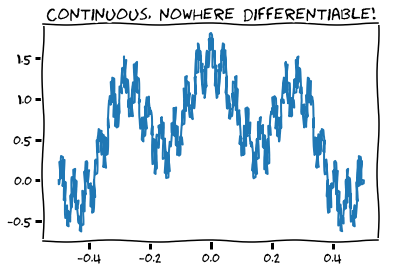
\includegraphics[width=0.6\linewidth]{weierstrass.png}
% \caption{Detail of the graph of $\mathcal{W}_{0.5, 7}$}
% \label{figure:WeierstrassFunction}
% \end{figure}
% \end{example}

% It is possible to extend the notion to higher derivatives.  We would say, for instance, that a function is \emph{twice differentiable} if the derivative is differentiable.  For the case of such a real-valued function $f \colon \field{R}^d \to \field{R}$, this would mean in particular that all second partial derivatives exist, and are continuous over the domain of $f$.

% We define for these functions the \emph{Hessian} of $f$ at $\x \in D$ to be the following matrix of second partial derivatives:
% \begin{equation*}
% \Hess{f}(\x) = \begin{bmatrix}
% \frac{\strut\partial^2 f}{\strut\partial x_1^2}(\x) & \frac{\strut\partial^2 f}{\strut\partial x_1 \partial x_2}(\x) &\dotsb &\frac{\strut\partial^2 f}{\strut\partial x_1 \partial x_d}(\x) \\
% &&&\\
% \frac{\strut\partial^2 f}{\strut\partial x_2 \partial x_1}(\x) & \frac{\strut\partial^2 f}{\strut\partial x_2^2}(\x) &\dotsb &\frac{\strut\partial^2 f}{\strut\partial x_2 \partial x_d}(\x) \\
% &&& \\
% \vdots & \vdots &\ddots &\vdots \\
% &&& \\
% \frac{\strut\partial^2 f}{\strut\partial x_d \partial x_1}(\x) & \frac{\strut\partial^2 f}{\strut\partial x_d \partial x_2}(\x) &\dotsb &\frac{\strut\partial^2 f}{\strut\partial x_d^2}(\x)
% \end{bmatrix}
% \end{equation*}